\selectlanguage{british}%

\chapter{Determinism Tests and Bohmian Mechanics}


\section{Rationale}

As was pointed out in the previous chapter, it is known that BM doesn't
assign a unique value to spin of a particle. For BM, spin is only
a property of the wavefunction. Recall that the GHZ test was formulated
for spins. Consequently, the conclusion that spins can't have pre-defined
values (deterministic) does not contradict BM outright. Precisely
how the GHZ test is compatible with BM, is worth exploring. It will
edify our understanding of how to analyse a physical situation using
BM and the relation between determinism \& non-locality. 

From the point of view of QM however, the treatment of spins is not
fundamentally different from that of phase-space variables (position
$q$ and momentum $p$). It is not surprising therefore, that the
GHZ test can be generalized to phase space and at least one such extension
is known \cite{GHZcontinuous}. The conclusion one draws from the
phase space GHZ test, would then be that $q,\,p$ can't have pre-defined
values. This then, is in direct contradiction with BM, which claims
that $q,\,p$ are precisely defined and their evolution completely
determined (given the initial position, $q_{0}$, and the wavefunction).
Since it is believed that BM is completely consistent with QM, it
is of considerable interest to explore how BM can resolve the apparent
paradox. If it fails, then we would have identified a way to falsify
BM.

\begin{comment}
We will find that to make predictions using BM, one requires knowledge
of the BM trajectory, which is not trivial to evaluate. Numerical
solutions are required to analyse most situations. 
\end{comment}



\section{GHZ}

For convenience, we recall that in our previous discussion, $\hat{A}\equiv\hat{\sigma}_{x}\otimes\hat{\sigma}_{y}\otimes\hat{\sigma}_{y}$,
$\hat{B}\equiv\hat{\sigma}_{y}\otimes\hat{\sigma}_{x}\otimes\hat{\sigma}_{y}$,
$\hat{C}\equiv\hat{\sigma}_{y}\otimes\hat{\sigma}_{y}\otimes\hat{\sigma}_{x}$,
and $\hat{D}\equiv\hat{\sigma}_{x}\otimes\hat{\sigma}_{x}\otimes\hat{\sigma}_{x}$,
which are such that $\hat{A}\left|\chi\right\rangle =\hat{B}\left|\chi\right\rangle =\hat{C}\left|\chi\right\rangle =\left|\chi\right\rangle $,
while $\hat{D}\left|\chi\right\rangle =-\left|\chi\right\rangle $,
for $\sqrt{2}\left|\chi\right\rangle =\left|000\right\rangle -\left|111\right\rangle $.


\subsection{Compatibility with BM}

To analyse any situation using BM, one is required to know the experimental
arrangement. In this case, we assume that spins are measured using
the Stern-Gerlach (SG) apparatus. Without loss of generality, let
us assume that the initial state of the particle is given by, $\sqrt{2}\left|\Psi(\vec{r}_{1},\vec{r}_{2},\vec{r}_{3},t=0)\right\rangle =\left|\psi_{+++}(\vec{r}_{1},\vec{r}_{2},\vec{r}_{3},t=0)\right\rangle \otimes\left|000\right\rangle -\left|\psi_{---}(\vec{r}_{1},\vec{r}_{2},\vec{r}_{3},t=0)\right\rangle \otimes\left|111\right\rangle $,
where $\vec{r}_{i}$ represents the position vector in the frame of
the $i^{th}$ observer. Note that the explicit tensor product is used
to separate the spin and position parts the three particles. If the
wavefunction for each particle is assumed to be Gaussian initially,
propogating along their respective axes of the SG apparatus, then
one can further simplify the form of $\left|\psi_{\pm\pm\pm}\right\rangle $.
It has been shown \cite{BohmGHZetc} that the time evolution of $\left|\psi_{\pm\pm\pm}\right\rangle $
can be written as products of 3 single particle solutions of the SG
setup, which was analyzed by Bohm himself. Once $\left|\Psi(\vec{r}_{i},t)\right\rangle $
is known, one can evaluate the equation of motion for the three particles,
using BM. If the SG apparatus are setup to measure say XYY, then from
both numerical simulations \& analysis of the trajectory equations,
the following is observed in the direction relevant to measurement.
Four attractor basins are formed: $(+++)$, $(+--)$, $(-+-)$, and
$(--+)$, where $\pm$ represent the physical location in the SG,
corresponding to a spin `up' (`down') measurement. The product is
always $+1$, consistent with predictions of QM. However, when the
SG apparatus are setup to measure XXX, the trajectories are found
to obey equations which possess four attractive basins: $(---)$,
$(-++)$, $(+-+)$ and $(++-)$. Again, the product is $-1$, in agreement
with QM. 

As a remark, it maybe stated, that the details of evaluating the trajectory,
become complicated rather quickly and that it is not trivial to obtain
analytic solutions for the phase-space scenario. Consequently, numerical
simulations are a necessity beyond this stage. (See \cite{BohmGHZetc}
for a flavour of the complexity)

In conclusion, one finds that non-locality enters the description
from the fact that the attractor basins which form, depend on the
settings of \emph{all} SG apparatus. Thus, we learn that while all
the results are deterministic, they depend on the precise experimental
setup, and not merely operators.


\subsection{Phase Space}

To extend the GHZ test to phase space, note first that we need only
the following situation. Consider instead of observables (which are
Hermitian), unitary operators, $\hat{X}$ and $\hat{Y}$ with the
following redefinitions: $\hat{A}\equiv\hat{X}^{\dagger}\otimes\hat{Y}\otimes\hat{Y}^{\dagger}$,
$\hat{B}\equiv\hat{Y}^{\dagger}\otimes\hat{X}^{\dagger}\otimes\hat{Y}$,
$\hat{C}\equiv\hat{Y}\otimes\hat{Y}^{\dagger}\otimes\hat{X}^{\dagger}$
and $\hat{D}=\hat{X}\otimes\hat{X}\otimes\hat{X}$. If these unitary
operators also satisfy $\{\hat{X},\hat{Y}\}=0=\{\hat{X},\hat{Y}^{\dagger}\}$,
then it follows that (a) $\hat{A}$, $\hat{B}$, $\hat{C}$ and $\hat{D}$
all commute and (b) $\hat{A}\hat{B}\hat{C}\hat{D}=-\mathbb{I}$. Now
any simultaneous eigenket of $\hat{A},\,\hat{B},\,\hat{C}$ and $\hat{D}$
will yield a GHZ situation. 

To see why that will work, replace the unitary operators with complex
numbers and note that the unitary property translates to each of these
numbers being uni-modular. Thus, $ABC=X^{*}\otimes X^{*}\otimes X^{*}$,
using $Y^{*}Y=1$ for each particle. This would entail that $ABC=D^{*}$,
viz. $ABCD=1$. However we also know that $ABCD=-1$, which yields
the contradiction.

Another patent issue with this scheme, is the use of unitary operators,
as opposed to observables. This issue is resolved by explicit construction,
however the idea can be motivated in general. If an arbitrary unitary
operator, is a function of some fixed observable, and that alone,
then one can measure the said observable. From this, the value of
the unitary operator can be evaluated, thereby dissolving the objection.


\subsubsection{Known Extension}

One possible construction \cite{GHZcontinuous}, involves the use
appropriate displacement operators. $\hat{X}\equiv e^{i\sqrt{\pi}\hat{q}/L}$
and $\hat{Y}\equiv e^{i\sqrt{\pi}\hat{p}L}$, where $L$ is some length
scale and units are s.t. $\hbar=1$ (for this section). These satisfy
$\{\hat{X},\hat{Y}\}=0$, which follows trivially by recalling that
$e^{i\hat{p}u}e^{i\hat{q}v}=e^{i\cancelto{1}{\hbar}uv}e^{i\hat{q}v}e^{i\hat{p}u}$.
To construct a simultaneous eigenstate, observe that for 
\begin{eqnarray*}
\sqrt{2}\left|\uparrow\right\rangle _{q_{0},p_{0}} & \equiv & \sum_{k=-\infty}^{\infty}e^{i\sqrt{\pi}2kp_{0}L}\left|q=\sqrt{\pi}L\left(q_{0}+2k\right)\right\rangle \\
 &  & +i\sum_{k=-\infty}^{\infty}e^{i\sqrt{\pi}(2k+1)p_{0}L}\left|q=\sqrt{\pi}L\left(q_{0}+2k+1\right)\right\rangle ,\\
\sqrt{2}\left|\downarrow\right\rangle _{q_{0},p_{0}} & \equiv & \sum_{k=-\infty}^{\infty}e^{i\sqrt{\pi}2kp_{0}L}\left|q=\sqrt{\pi}L\left(q_{0}+2k\right)\right\rangle \\
 &  & -i\sum_{k=-\infty}^{\infty}e^{i\sqrt{\pi}(2k+1)p_{0}L}\left|q=\sqrt{\pi}L\left(q_{0}+2k+1\right)\right\rangle ,
\end{eqnarray*}
where $p_{0}L/\sqrt{\pi}$ \& $\sqrt{\pi}Lq_{0}$ $\in[0,1)$, $\hat{X}\left|\uparrow\right\rangle =\left|\downarrow\right\rangle $,
$\hat{Y}\left|\uparrow\right\rangle =i\left|\downarrow\right\rangle $
and similarly $\hat{X}\left|\downarrow\right\rangle =\left|\uparrow\right\rangle $,
$\hat{Y}\left|\downarrow\right\rangle =-i\left|\uparrow\right\rangle $
(we have dropped $q_{0}$ and $p_{0}$ for simplicity). This also
holds for $\hat{X}^{\dagger}$ and $\hat{Y}^{\dagger}$. To see this,
note that $\hat{Y}^{\dagger}\left|q\right\rangle =\left|q+\sqrt{\pi}L\right\rangle $
while $\hat{X}\left|x\right\rangle =e^{i\sqrt{\pi}q/L}\left|q\right\rangle $.
If one defines $\hat{Z}=i\hat{Y}\hat{X}$, from the aforesaid, it
follows $\hat{Z}\left|\uparrow\right\rangle =\left|\uparrow\right\rangle $
and $\hat{Z}\left|\downarrow\right\rangle =-\left|\downarrow\right\rangle $.
The problem has been made sufficiently analogous to the original GHZ
test. It is now immediate that the required simultaneous entangled
eigenket must be 
\[
\left|\psi\right\rangle =\frac{\left|\uparrow\uparrow\uparrow\right\rangle -\left|\downarrow\downarrow\downarrow\right\rangle }{\sqrt{2}}.
\]
It is obvious that for obtaining the value of $\hat{X}$, one need
only measure $\hat{q}$ and $\hat{p}$ to obtain the value of $\hat{Y}$
and their conjugates. We have therefore an extension of the GHZ test
to continuous variables. To understand how BM explains this however,
one must be able to simulate this. The test in the given form, is
not simple to simulate, since the states involved have infinite spread
in position space (infact one can show that even in momentum space
the spread is infinite). Further, the wavefunction in position space,
is a countable union of disjoint delta functions. Neither of these
are desired from the numerical point of view. The latter can be handled
by integrating $\left|\uparrow\right\rangle _{q_{0},p_{0}}$ over
$q_{0}$ with an appropriate weight. However, no simple way could
be conceived of to suppress the infinite spread.


\subsubsection{Optimized Extension \label{sub:Optimized-Extension}}

This result was obtained after considerable effort. We construct an
optimization of the phase space GHZ test, such that (a) the wavefunctions
aren't sharp (no delta functions) and (b) that they disappear as $q\to\pm\infty$.
We consider the same states $\left|\psi_{0}\right\rangle ,\left|\psi_{1}\right\rangle $
for $N=2M=8$, as those considered in \cite{BellMacroscopic}. These
are given by 
\[
\left|\psi_{0}\right\rangle \equiv\frac{1}{\sqrt{M}}\sum_{n=-\lfloor\frac{M}{2}\rfloor}^{\lfloor\frac{M-1}{2}\rfloor}\left|\varphi_{2n+1}\right\rangle ,\,\left|\psi_{1}\right\rangle \equiv\frac{1}{\sqrt{M}}\sum_{n=-\lfloor\frac{M}{2}\rfloor}^{\lfloor\frac{M-1}{2}\rfloor}\left|\varphi_{2n}\right\rangle ,
\]
where $\varphi(q)=\left\langle q|\varphi\right\rangle $ is a localized
state, symmetric about $q=L/2$, where $L$ is some length scale and
$\varphi_{n}(q)\equiv\varphi(q-nL)$ and $M$ characterizes the `size'
of the state (see \prettyref{fig:Illustration-of-multicomponent}).
\begin{figure}
\begin{centering}
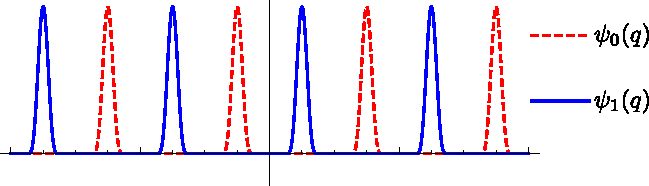
\includegraphics[width=0.7\textwidth]{Chapter2/Figs/Vector/ghzOpt}
\par\end{centering}

\caption{Illustration of multicomponent superposition states $\left|\psi_{0}\right\rangle $
and $\left|\psi_{1}\right\rangle $ for $N=8$ \cite{BellMacroscopic},
used in the optimization of the GHZ test.\label{fig:Illustration-of-multicomponent}}


\selectlanguage{english}%
\selectlanguage{english}%
\end{figure}
For $\hat{Z}\equiv Z(\hat{q})=\text{sgn}(\sin(\hat{q}\pi/L))$, we
have $\hat{Z}\left|\psi_{0}\right\rangle =\left|\psi_{0}\right\rangle $
and $\hat{Z}\left|\psi_{1}\right\rangle =-\left|\psi_{1}\right\rangle $.
In addition to this, we define $\hat{X}=e^{-i\hat{p}L/\hbar}$ (note
that this is not Hermitian). Observe that $\left|\psi_{\pm}\right\rangle \equiv\frac{\left|\psi_{0}\right\rangle +\left|\psi_{1}\right\rangle }{\sqrt{2}}$
is not an eigenstate of $\hat{X}$, although it comes close. We optimize
the observable $\hat{X}$ to $\hat{X}'\equiv\hat{X}\hat{T}$, where
$\hat{T}\equiv e^{i\hat{p}NLa(\hat{q})/2}$ and 
\[
a(q)=\begin{cases}
1 & 2L<q<4L\\
0 & \text{else}
\end{cases}.
\]
The idea is that you shift certain peaks to the right place, before
applying the displacement operator $\hat{X}$. To illustrate this,
consider explicitly $\left|\psi_{0}\right\rangle =\left(\left|\varphi_{-4}\right\rangle +\left|\varphi_{-2}\right\rangle +\left|\varphi_{-1}\right\rangle +\left|\varphi_{-3}\right\rangle \right)/\sqrt{4}$.
The operation of $\hat{T}$ is $\hat{T}\left|\varphi_{4}\right\rangle =\left|\varphi_{-5}\right\rangle $,
$\hat{T}\left|\varphi_{3}\right\rangle =\left|\varphi_{-6}\right\rangle $
and $\hat{T}\left|\varphi_{n}\right\rangle =\left|\varphi_{n}\right\rangle $
for $n\in\{-4,-3,-2,-1,1,2\}.$ It is now evident that $\hat{X}'=\hat{X}\hat{T}\left|\psi_{0}\right\rangle =\left|\psi_{1}\right\rangle $.
Note also that $\hat{X}'^{\dagger}\left|\psi_{0}\right\rangle =\left|\psi_{1}\right\rangle $.
Similarly $\hat{X}'\left|\psi_{1}\right\rangle =\left|\psi_{0}\right\rangle $
and $\hat{X}'^{\dagger}$ does the same. So finally, consider $\left|\psi_{G}\right\rangle \equiv\left(\left|\psi_{0}\psi_{0}\psi_{0}\right\rangle -\left|\psi_{1}\psi_{1}\psi_{1}\right\rangle \right)/\sqrt{2}$.
With $\hat{A}\equiv\hat{X}'\otimes\hat{Y}'\otimes\hat{Y}'^{\dagger}$,
where $\hat{Y}'\equiv i\hat{Z}\hat{X}'$, calculations yield $\hat{A}\left|\psi_{G}\right\rangle =\left|\psi_{G}\right\rangle $.
With $\hat{B}\equiv\hat{Y}'^{\dagger}\otimes\hat{X}'\otimes\hat{Y}'$
and $\hat{C}\equiv\hat{Y}'\otimes\hat{Y}'^{\dagger}\otimes\hat{X}'$
also, by symmetry we get $\hat{B}\left|\psi_{G}\right\rangle =\left|\psi_{G}\right\rangle $
and $\hat{C}\left|\psi_{G}\right\rangle =\left|\psi_{G}\right\rangle $.
Now $\hat{E}\equiv\hat{A}\hat{B}\hat{C}=\hat{X}'\otimes\hat{Y}'\hat{X}\hat{Y}'^{\dagger}\otimes\hat{X}'$
and $\hat{D}\equiv\hat{X}'\otimes\hat{X}'\otimes\hat{X}'$ yield the
paradox. If values were predefined, the value of $\hat{D}$ and $\hat{E}$
would return the same answer. However, a simple calculation yields
$\hat{E}\left|\psi_{G}\right\rangle =\left|\psi_{G}\right\rangle $
(this can be seen directly by applying $\hat{A},\,\hat{B}$ and $\hat{C}$
sequentially on $\left|\psi_{G}\right\rangle $), while $\hat{D}\left|\psi_{G}\right\rangle =-\left|\psi_{G}\right\rangle $.

The wavefunction now satisfies both the conditions required. The cost
that one pays however, is that a simple measurement of $\hat{q}$
and $\hat{p}$ won't suffice. It remains to see precisely which observable
one must measure and what must be the analogue of the SG apparatus.


\section{BM Simulator \label{sec:BM-Simulator}}

Simulation of BM is a two step process. First one must be able to
simulate QM, viz. the Schr\"odinger equation and second, be able
to evaluate the position of the particle at each time step. 


\subsection{Design of Numerics}

The code was written in Fortran, due to it's efficacy at handling
arrays, in conjunction with gnuplot. Runge Kutta 4 was used to solve
the differential equations and spline interpolation was used for calculating
velocities of the particle. Initial goal was simply to find the trajectories
for a single particle, with only one degree of freedom.


\subsubsection{Simulation of Schr\"odinger's Equation}

To simulate a differential equation, say $\dot{q}=f(q)$, one obvious
method is to simply use $q_{n+1}=q_{n}+f(q_{n})\Delta t$, $t_{n+1}=t_{n}+\Delta t$
where $n$ parametrizes the sequence and $\Delta t$, the time step.
To get reasonably accurate results, one needs to keep $\Delta t$
small. This is known as the Euler method and it has errors of $\mathcal{O}(\Delta t^{2})$.
However, there's another known method, popularly referred to as ``RK4'',
short for Runge Kutta 4, which has errors of $\mathcal{O}(\Delta t^{5})$.
Assuming again that $\dot{q}=f(q)$, the method claims that $q_{n+1}=q_{n}+\frac{h}{6}(k_{1}+2k_{2}+2k_{3}+k_{4})$,
$t_{n+1}=t_{n}+h$, where 
\begin{eqnarray*}
k_{1} & = & f(q_{n}),\\
k_{2} & = & f(q_{n}+hk_{1}/2),\\
k_{3} & = & f(q_{n}+hk_{2}/2),\\
k_{4} & = & f(q_{n}+hk_{3}),
\end{eqnarray*}
and $h=\Delta t$. The derivation is tangential to our interest and
will have to be skipped. The advantage is that this method can produce
accurate results for relatively larger $\Delta t$ also. 

Our purpose is to solve the Schr\"odinger Equation, viz. $\partial\psi/\partial t=-(\hbar^{2}/2m)(\partial^{2}\psi/\partial q^{2})+V(q)\psi$.
Clearly this is more complicated than the case discussed before, for
now we have to solve for $\psi$, and $\psi$ is a function of both
$q$ and $t$. We begin with uniformly discritizing $\psi$ in the
position space, so that $\psi$ is known only at finite points $\{q_{n}\}$
to start with (and has spacing $\Delta q$), while time is discritized
as usual, with step $\Delta t$. Imagine that we are at the $n^{th}$
step, $q_{i}$ and $t_{n}$ are known, and so is $\psi_{n}(\{q_{i}\})$
(where the notation means that at the $n^{th}$ step, $\psi_{n}$
is known at all the points $\{q_{i}\}$). Given $\psi_{n}(\{q_{i}\})$,
one can evaluate $\partial^{2}\psi/\partial q^{2}=\psi''$ using the
definition of the derivitive, without imposing the $h\to0$ limit
(in the usual notation) and obtain $\psi''(q_{i})=\left[\psi(q_{i+1})-2\psi(q_{i})+\psi(q_{i-1})\right]/(\Delta q)^{2}$.
The objective is to find $\psi_{n+1}(q_{i})$, which according to
the Euler method can be evaluated as $\psi_{n+1}(q_{i})=\left[-\psi''(q_{i})+V(q_{i})\psi\right]\Delta t$,
where for illustration, we have set $\hbar^{2}/2m=1$. Practically
this doesn't suffice and we are forced to use RK4 (or any better alternative).
To use RK4, one must be careful and remember that we are evaluating
$\psi$ for a given value $q_{i}$. Therefore in the evaluations of
$k_{i}$, $q_{i}$ must be kept fixed, for here $\psi$ is the variable,
playing the role of $q$. Ofcourse, $\psi$ is a complex variable
Accordingly, we must have, suppressing $q_{i}$ to avoid confusion,
$\psi_{n+1}=\psi_{n}+\frac{h}{6}(k_{1}+k_{2}+k_{3}+k_{4})$, where
\begin{eqnarray*}
k_{1} & = & -\psi_{n}''+V\psi_{n},\\
k_{2} & = & -(\psi_{n}+hk_{1}/2)''+V(\psi_{n}+hk_{1}/2),\\
k_{3} & = & -(\psi_{n}+hk_{2}/2)''+V(\psi_{n}+hk_{2}/2),\\
k_{4} & = & -(\psi_{n}+hk_{3})''+V(\psi_{n}+hk_{3}),
\end{eqnarray*}
and $h=\Delta t$. Let us take a moment to understand how one must
go about evaluating this numerically. Since $\psi_{n}''(q_{i})$ and
$\psi_{n}(q_{i})$ are known, one can evaluate $k_{1}(q_{i})$ trivially.
To evaluate $k_{2}(q_{i})$ however, we would require $k_{1}(\{q_{i}\})$
to be known (or at least $k_{1}(q_{i-1})$, $k_{1}(q_{i})$ and $k_{1}(q_{i+1})$).
Thus, we first evaluate $k_{1}$ $\forall\,q_{i}$ in the grid. Then
to evaluate $k_{2}(q_{i})$, we need $(\psi_{n}+hk_{1}/2)''$, evaluated
at $q_{i}$. Since the finite difference method requires it's argument
to be known at $q_{i-1}$, $q_{i}$ and $q_{i+1}$, we see that knowing
$k_{1}(\{q_{i}\})$ is sufficient to evaluate this step. One similarly
evaluates $k_{2}(\{q_{i}\})$ to evaluate $k_{3}(\{q_{i}\})$ and
then $k_{4}(\{q_{i}\})$. It maybe added as remark, that practically
it is found, that $\Delta t/\Delta x^{2}\le10^{-6}$ or so for Euler
and $10^{-4}$ or so for RK4, as was also pointed out by \cite{schrNum}.
The aforesaid was observed to successfully simulate the Schr\"odinger
equation, for a variety of potentials, details of which follow.


\subsubsection{Simulation of trajectories}

According to Bohmian Mechanics, $\dot{q}=p/m=\nabla S/m=\hbar\text{Im}(\nabla\psi/\psi)$,
where $\psi=Re^{iS/\hbar}$. From the previous section, we have $\psi_{n}$,
discretized $\psi$ at each time step. We conclude therefore, that
the simplest way to obtain $\nabla S$ at an arbitrary position, is
to interpolate $\psi$ and subsequently evaluate $\nabla S$. Spline
interpolation is quite standard and fairly simple to extend to complex
variables. The details will not be discussed here, but the code written
{[}see \prettyref{sub:BM-Simulation-Results}{]} can be referred to.
It maybe mentioned that given $\psi(\{q_{i}\})$, one can evaluate
spline co-efficients, using which, one can easily (in a computationally
cheap way) evaluate $\psi(q)$ for practically any value of $q$.
To evolve $q$, viz. to obtain $q_{n}$, again RK4 was used where
this time, there are no complications. To be able to better appreciate
the results, one needs to plot multiple trajectories simultaneously.
The mildly non-trivial aspect of this part, is that one needs to start
with particles distributed according to $|\psi|^{2}$. Attempts were
made to find a library that can do this, but with no luck. A method
to convert a uniform random distribution to an arbitrary distribution
was independently arrived at, for a course on Numerical Methods. The
idea was to use a uniform random generator, with range $[0,1]$, which
for the $j^{th}$ particle, yields $c^{(j)}$, say. The method is
that, from the cumulative $\phi(q)=\int_{-\infty}^{q}\left|\psi(q')\right|^{2}dq'$
, one finds $q^{(j)}$ s.t. $\phi(q^{(j)})=c^{(j)}$, viz. $q^{(j)}=\phi^{-1}(c)$.
The inverse is guaranteed to be single valued, because the cumulative
is monotonically increasing. While a formal proof can be presented,
we will satisfy ourselves with noting the following. Intuitively,
a range of positions with high probability, will cause a larger range
of $c$ values to yield those positions, making them more likely to
appear; since all values of $c$ are equally likely. With all these
ingredients combined, Bohmian trajectories were successfully simulated.


\subsection{Performance against analytic results}

Three known physical situations were tested. (a) $V=0$; It is known
that a Guassian under free evolution, simply expands. (b) $V=\frac{1}{2}\omega^{2}q^{2}$;
It is known that a displaced Gaussian, oscillates under a harmonic
potential (see \prettyref{fig:Simulated-Bohmian-Trajectories}), and
so does it's spread (unless a coherent state is chosen). (c) Double
slit; By using a time varying potential, s.t. 
\[
V=\begin{cases}
0 & t\le t_{a}\\
V_{\text{dw}} & t_{a}<t\le t_{b}\\
0 & t_{b}<t
\end{cases}
\]
where $V_{\text{dw}}(q)$ represents two wells, simulating the double
slit effect, with a single degree of freedom.

In all cases, the results were qualitatively found to match. In case
of the double slit, although the wavefunction intereference pattern
was distorted, one could see the particles preferentially collecting
at the maxima. 

\begin{figure}
\begin{centering}
\subfloat{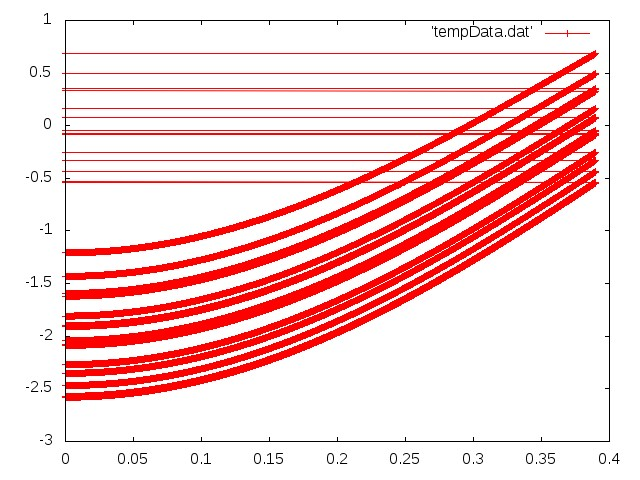
\includegraphics[width=0.3\columnwidth]{Chapter2/Figs/Raster/harmonic1.jpeg}}~~~\subfloat{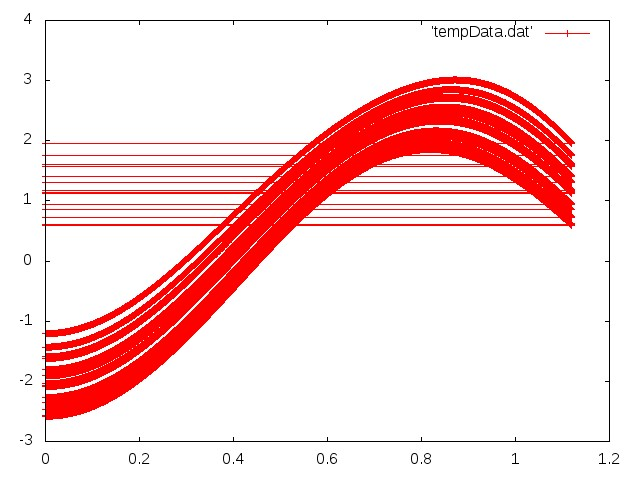
\includegraphics[width=0.3\columnwidth]{Chapter2/Figs/Raster/harmonic2.jpeg}}~~~\subfloat{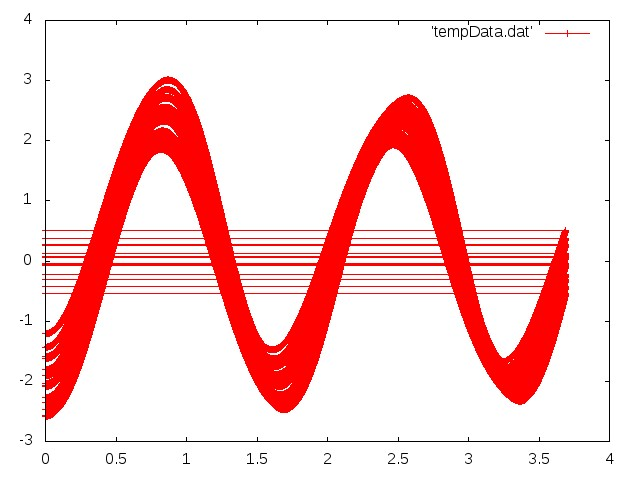
\includegraphics[width=0.3\columnwidth]{Chapter2/Figs/Raster/harmonic.jpeg}}
\par\end{centering}

\caption{Simulated Bohmian trajectories for a harmonic oscillator.\label{fig:Simulated-Bohmian-Trajectories}}


\selectlanguage{english}%
\selectlanguage{english}%
\end{figure}



\subsection{Simulation Results\label{sub:BM-Simulation-Results}}

BM was successfully simulated for a particle, with a single degree
of freedom, influenced by an arbitrary potential. Implementing RK4,
interpolation and random distribution generation were among the non-trivial
aspects. Generalization to multiple particles and inclusion of spins,
was among the immediate next steps, however due to later theoretical
developments, were not carried out. The code is available at \cite{gitHubThesisSim}
%\href{https://github.com/toAtulArora/msThesis/tree/master/numerics}{github.com/toAtulArora/msThesis/tree/master/numerics}.


\section{Measurements in BM (I)\label{sec:Measurements-in-BM}}

Measurement of spins in BM was discussed in the previous chapter.
Our interest in this chapter, is in measuring $q$, $p$ and functions
there of. We will learn that one can infact construct a universal
method that facilitates the measurement of any arbitrary observable.
The analysis will clarify two notions which are at high risk of being
misconstrued. First, that the position of the particle, when measured,
will infact yield $q$. However, a measurement of momentum of a particle,
as we will see, does not always yield $p$ (the value it had prior
to measurement). Infact, it would be inconsistent with QM if it did;
for instance, consider $\psi(q)=\left(1/\sqrt{\pi}\right)e^{-q^{2}}$,
for which $S=0$ and therefore so is $p=\nabla S=0$. However it is
known that upon measurement of momentum, one obtains a distribution
given by the fourier transform of $\psi$. Although this is centred
around the origin, it is not a delta function (has non-zero spread).
The second notion which is clarified, is that to find the value obtained
upon measurement of certain observables, knowledge about the precise
position of the measuring particle (the particle used to make the
measurement) can play a deciding role.


\subsection{Observable with discrete spectrum | Hamiltonian Approach}

Bohm has discussed in his second paper \cite{Bohm2}, how any arbitrary
observable maybe measured, in BM. To describe a measurement, we use
a measuring particle (mass $m_{L}$, say), by getting it to interact
with the system for a short duration appropriately. Subsequently,
we measure the final position of the particle, to learn about the
value of the observable of interest. Say for instance, we wish to
measure the observable $\hat{L}$, then the required interaction Hamiltonian
is given by $\hat{H}_{\text{int}}=a\hat{L}\otimes\hat{p}$. Here the
first operator acts on the system and second (after the tensor product
symbol) acts on the measuring particle. $a$ quantifies the interaction
strength. It has dimensions of frequency, if $L$ has dimensions of
length. Let us assume that the system in the state $\left|\psi\right\rangle $.
Then it is known that one can express $\left|\psi\right\rangle =\sum_{l}\left\langle l|\psi\right\rangle \left|l\right\rangle $,
where $\left|l\right\rangle $ are the eigenstates of $\hat{L}$ with
eigenvalue $l$ (we have assumed non-degenercy for simplicity, but
its removal doesn't cause any significant difficulty). $\left|\Psi_{S}(t)\right\rangle =\hat{U}(t)\left|\psi\right\rangle \otimes\left|\varphi\right\rangle $,
where 
\[
\hat{U}(t)=e^{-\frac{i}{\hbar}\left[-\hbar^{2}\frac{\nabla_{1}^{2}}{2m}-\hbar^{2}\frac{\nabla_{2}^{2}}{2m_{L}}+\hat{H}_{\text{int}}\right]t}
\]
 and $\left|\varphi\right\rangle $ is the state of the measuring
particle, given by a Guassian centred at the origin, $\varphi(q)=(1/\sqrt{2\pi}\sigma)e^{-q^{2}/2\sigma^{2}}$.
If $t$ is very small, and $a$ very large, s.t. $at=\lambda$ is
a finite number, then one can neglect the free evolution, $\nabla^{2}t$
terms compared to $\hat{H}_{\text{int}}t$. We then have 
\begin{eqnarray*}
\left|\Psi_{S}(t)\right\rangle  & = & e^{-\frac{i}{\hbar}a\hat{L}\otimes\hat{p}t}\left|\Psi_{S}\right\rangle \\
 & = & \sum_{l}\left\langle l|\psi\right\rangle \left|l\right\rangle \otimes e^{-\frac{i}{\hbar}\lambda l\,\hat{p}}\left|\varphi\right\rangle \\
 & = & \sum_{l}\left\langle l|\psi\right\rangle \left|l\right\rangle \otimes\left|\varphi_{\lambda l}\right\rangle ,
\end{eqnarray*}
where $\left|\varphi_{q_{0}}\right\rangle =\int dq\varphi(q-q_{0})\left|q\right\rangle $.
This interaction, effectively entangles the measuring particle, with
the possible `outcomes', eigenstates of the observable $\hat{L}$
of interest. If $\sigma\ll\lambda l$, then according to QM itself,
a position measurement of the measuring particle, would correspond,
in a one-to-one way, to the eigenstate/eigenvalue of $\hat{L}$, to
which the system will collapse. In the context of BM, after the interaction,
the measuring particle would be guided into one of these eigenstates,
and a position measurement would yield the same. We glossed over various
details in making the last statement, which will be delineated shortly,
through some illustrations. 


\subsubsection{Generalization to observables with continuum spectrum \label{sub:BM-measurement-to-continuous}}

Since we are interested in observing phase space variables, the aforesaid
must be generalized to the continuous spectrum regime. We proceed
with the aforesaid notation, and promote the discrete operator $\hat{L}$
to have a continuous spectrum. Thus $\left|\psi\right\rangle =\int dl\left\langle l|\psi\right\rangle \left|l\right\rangle $,
and recall $\left|\varphi\right\rangle =\int dq\varphi(q)\left|q\right\rangle $,
where $\varphi(q)$ has $\sigma$ quantifying the deviation from the
origin. Now $\left|\Psi_{S}(t)\right\rangle =\hat{U}(t)\left|\psi\right\rangle \otimes\left|\varphi\right\rangle =\int\int dldq\varphi(q)\left\langle l|\psi\right\rangle \left|l\right\rangle \otimes\left|q+l\lambda\right\rangle $,
where $\lambda=at$ as before. Say $q$ is measured at this stage
and $q'$ is the value obtained. The resultant state would then be
$\left|q'\right\rangle \left\langle q'\right|\left|\Psi_{S}\right\rangle =\int\int dldq\varphi(q-l\lambda)\left\langle l|\psi\right\rangle \left|l\right\rangle \delta(q-q')=\int dl\varphi(q'-l\lambda)\left\langle l|\psi\right\rangle \left|l\right\rangle $.
We know that $\varphi(q)\approx0$ when $q\notin(-\delta q,\delta q)$,
where $\delta q=\mathcal{O}(\sigma)$ can be chosen, depending on
the accuracy desired. This implies $-\delta q<q'-l\lambda<\delta q$,
which entails that $l=\frac{q'}{\lambda}\pm\frac{\delta q}{\lambda}$.
We thus have a relation between the observed position, $q'$, of the
measuring particle, and the value of the operator $\hat{L}$. The
error is controlled by the sharpness of the initial state of the measuring
particle.


\subsubsection{Consistency check; measurement of position \label{sub:BM-Consistency-check-measurement}}

The position of a particle, as is claimed by BM, remains the same
upon observing. Let us verify this statement, by applying the aforesaid
formalism. For simplicity, let us assume that the state of the system
is given as $\sqrt{2}\left|\psi\right\rangle =\int dq\left[\delta(q-q_{0})+\delta(q+q_{0})\right]\left|q\right\rangle $,
which is to say, the system is in a superposition of being at $q_{0}$
and $-q_{0}$. Let us assume that the particle is initially given
to be in $q_{1}=q_{0}$. Now our measurement formalism must be consistent
with this, viz. the answer must not depend on the initial position
of the measuring particle. Initially then, the state is $\left|\Psi_{S}\right\rangle =\left|\psi\right\rangle \otimes\left|\varphi\right\rangle $,
while after interaction, the state becomes $\sqrt{2}\left|\Psi_{S}(t)\right\rangle =\left|q_{0}\right\rangle \otimes\left|\varphi_{\lambda q_{0}}\right\rangle +\left|-q_{0}\right\rangle \otimes\left|\varphi_{-\lambda q_{0}}\right\rangle $.
To understand this clearly, one must plot $\left|\Psi_{S}(q_{1},q_{2})\right|^{2}=\left|\left\langle q_{1},q_{2}|\Psi_{S}\right\rangle \right|^{2}$,
where $\left|q_{1}\right\rangle $ is (the position eigenket) for
the system and $\left|q_{2}\right\rangle $ for the measuring particle.
\begin{figure}
\begin{centering}
\subfloat[Before interaction\label{fig:PosMes-Before-interaction}]{\begin{centering}
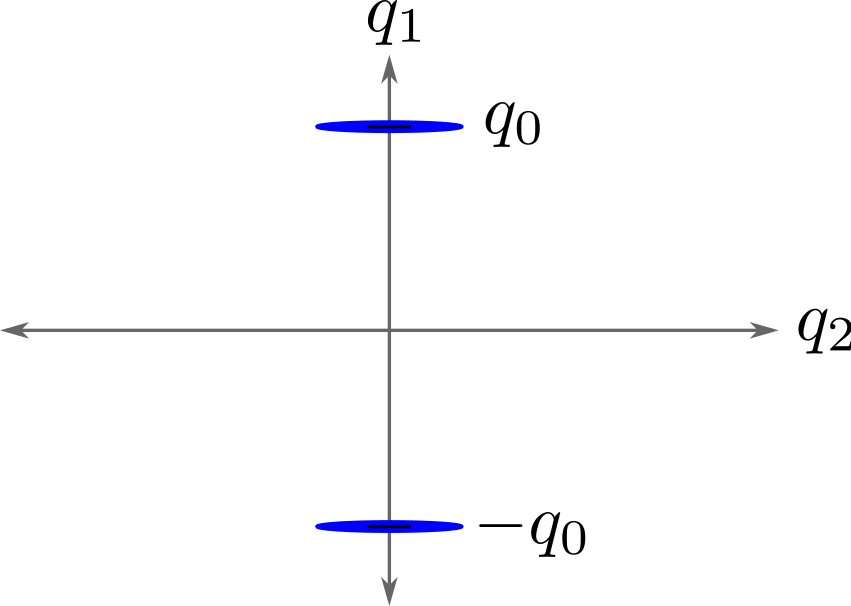
\includegraphics[width=0.45\textwidth]{Chapter2/Figs/Raster/posMesBefore}
\par\end{centering}

\selectlanguage{english}%
\selectlanguage{english}%
}~~ ~~\subfloat[After interaction\label{fig:PosMes-After-interaction}]{\begin{centering}
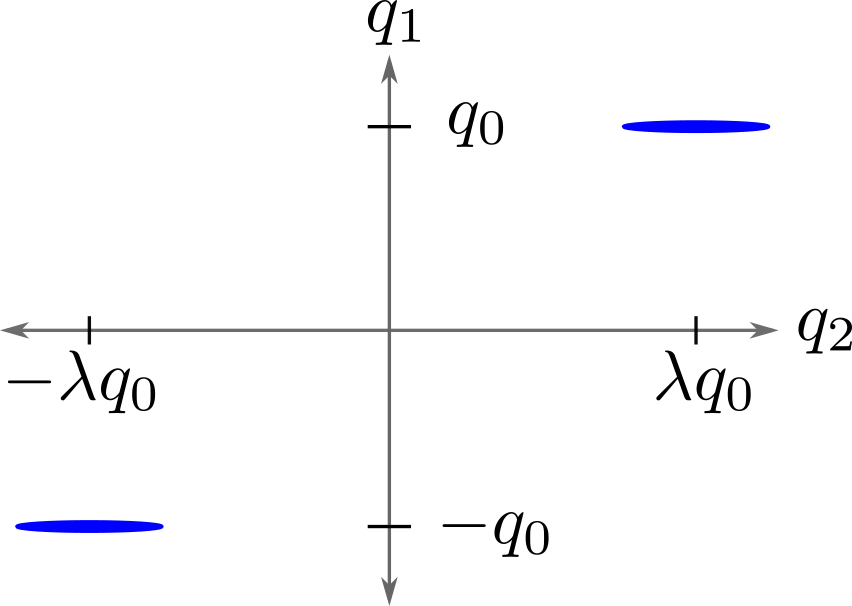
\includegraphics[width=0.45\textwidth]{Chapter2/Figs/Raster/posMesAfter}
\par\end{centering}



\selectlanguage{english}%
\selectlanguage{english}%
}
\par\end{centering}

\caption{Indicative contour plot of $\left|\left\langle q_{1},q_{2}|\Psi_{S}\right\rangle \right|^{2}$,
illustrating consistency of position measurements. }


\selectlanguage{english}%
\selectlanguage{english}%
\end{figure}
Before the interaction (see \prettyref{fig:PosMes-Before-interaction}),
say the measuring particle was at $q_{2}\in(-\sigma,\sigma)$. After
the interaction (see \prettyref{fig:PosMes-After-interaction}), the
measuring particle will move to $q_{2}\in(\lambda q_{0}-\sigma,\lambda q_{0}+\sigma)$,
which follows simply by noting that the velocities are given by probability
current. A measurement of the particle's position would yield $q_{2}\approx\lambda q_{0}$,
which we know from our analysis, corresponds to $q_{1}=q_{0}$, which
is infact consistent with our initial conditions. It must be emphasized
that the position of the measuring particle, plays no essential role
in deciding where it would show up. The same analysis can be repeated
for $q_{1}=-q_{0}$ and in this case, from \prettyref{fig:PosMes-After-interaction},
it would follow that after the interaction, $q_{2}\approx-\lambda q_{0}$.
Consistency of this method is therefore established. Ofcourse, one
can relax the idealized $\delta$ functions to obtain more realistic
functions, but the conclusion remains invariant.


\subsubsection{Consistency check; measurement of momentum}

We now resolve the issue pointed out in the beginning of this section,
viz. the observed value of $p$ being inconsistent with QM. We begin
with writing the state of the system as $\left|\psi\right\rangle =\int dq\left(1/\sqrt{\pi}\right)e^{-q^{2}}\left|q\right\rangle $,
so that $p=\nabla S=0$. We wish to find, how the spread in the observed
value of $p$ appears, from the aforesaid measurement formalism. Note
that 
\begin{eqnarray*}
\left|\psi\right\rangle  & = & \int dp\left|p\right\rangle \int dq\cancelto{\left(1/\sqrt{2\pi\hbar}\right)e^{-iqp/\hbar}}{\left\langle p|q\right\rangle }\psi(q)\\
 & = & \int dp\tilde{\psi}(p)\left|p\right\rangle ,
\end{eqnarray*}
where $\tilde{\psi}(p)$ is $\psi(q)$ fourier transformed. The combined
state before measurement is given by $\left|\Psi_{S}\right\rangle =\left|\psi\right\rangle \otimes\left|\varphi\right\rangle $,
while after the measurement, $\left|\Psi(t)\right\rangle =\int dp\tilde{\psi}(p)\left|p\right\rangle \otimes\left|\varphi_{\lambda p}\right\rangle $.
The aforesaid expression entails that, assuming $\sigma\to0$, the
probability for the measuring particle, to end up at $\lambda p$,
is given by $\left|\tilde{\psi}(p)\right|^{2}$, which is consistent
with QM. To obtain this result more carefully from Bohmian trajectories,
one must plot $\left|\left\langle q_{1},q_{2}|\Psi_{S}\right\rangle \right|^{2}$
as was done in the previous section, but we will satisfy ourselves
here, with noting that the measurement process has explicitly imparted
momentum on the system, as is clear after `collapsing' the wavefunction.


\subsection{Classical limit of measurements}

Although we have not yet discussed the classical limit of BM, as an
aside, it maybe demonstrated that this indeed follows elegantly. If
we write $\psi=Re^{iS/\hbar}$ and substitute this in the Schr\"odinger
Equation, and separate the real and imaginary parts, we obtain 
\begin{eqnarray*}
\frac{\partial R}{\partial t} & = & -\frac{1}{2m}\left[R\nabla^{2}S+2\nabla R.\nabla S\right],\\
\frac{\partial S}{\partial t} & = & -\left[\frac{\nabla S^{2}}{2m}+V-\frac{\hbar^{2}}{2m}\frac{\nabla^{2}R}{R}\right].
\end{eqnarray*}
The reader would've recognized that the second equation is essentially
the Hamilton Jacobi equation, with an extra term. Infact, if one writes
$P=R^{2}$, then we obtain 
\begin{eqnarray*}
\frac{\partial P}{\partial t}+\nabla.\left(P\frac{\nabla S}{m}\right) & = & 0\\
\frac{\partial S}{\partial t}+\frac{\nabla S^{2}}{2m}+V-\frac{\hbar^{2}}{4m}\left[\frac{\nabla^{2}P}{P}-\frac{1}{2}\frac{\nabla P^{2}}{P^{2}}\right] & = & 0
\end{eqnarray*}
which makes the first equation effectively a continuity equation for
probabilities, if one relates $\nabla S=p$ (momentum in BM), as is
done in the Hamilton Jacobi framework. Effectively then, BM elegantly
yields the classical limit, for if we neglect the $\hbar$ term, then
we have particles obeying Newton's laws. 

Our motivation was to study how the measured value of momentum turns
out to be $p=\nabla S$ in the classical limit. The larger goal, was
to use this elegant framework, to understand how measurement of functions
of $q,\,p$, such as the energy for example, become equivalent to
measuring $q$ and $p$ and plugging their values into the function.
To be precise, consider the example of an energy eigenstate in a harmonic
potential. For this state, neither $q$ nor $p$ are precisely defined
(in the language of QM), however, the energy is sharp. We started
with analysing the classical limit of the measurement process, just
discussed. That requires the potential $V$, to be a function of both
$q$ and $p$, whereas for the aforesaid derivation, only position
dependent $V$ was used. Correcting for this, create various issues.
First of all, this interaction adds a term to the continuity equation,
\[
\frac{\partial P}{\partial t}+\nabla_{1}\left(P\frac{\nabla_{1}S}{m}\right)+\nabla_{2}\left(P\frac{\nabla_{2}S}{m}\right)+\overbrace{2aR\left[\nabla_{1}R\nabla_{2}S+R\nabla_{1}\nabla_{2}S+\nabla_{2}R\nabla_{1}S\right]}^{\text{Extra Term! | How will}\,P\,\text{satisfy the continuity equation?}}=0.
\]
The interaction also adds a ``quantum potential'' in addition to the
expected potential, which doesn't seem to disappear in the large mass
limit, 
\[
\frac{\partial S}{\partial t}+\frac{(\nabla_{1}S)^{2}}{2m}+\frac{(\nabla_{2}S)^{2}}{2m}+\overbrace{a\nabla_{1}S\nabla_{2}S}^{\text{expected part}}-\overbrace{a\hbar^{2}\frac{\nabla_{1}\nabla_{2}R}{R}}^{\text{\text{quantum part}}}-\underbrace{\frac{\hbar}{2mR}(\nabla_{1}^{2}R+\nabla_{2}^{2}R)}_{\text{usual quantum potential}}=0.
\]
One can see that with $\hbar\to0$, the quantum potential and the
quantum part of the interaction, both disappear. However, the continuity
equation is not recovered still. This part was not explored further,
but can perhaps be studied independent of our current target.


\subsection{Measurement Exploration Summarized}

From the optimized GHZ construction, it was necessary to arrive at
a theoretical construction, that would allow calculation of measurement
outcomes associated with arbitrary operators composed using $\hat{q},\,\hat{p}$.
This was achieved, however it was found that obtaining these results
is not trivial in most cases of interest. The surprising result, that
measurement of $\hat{p}$ may not yield $p=\nabla S$, while a measurement
of $\hat{q}$ yields $q$, was derived and clarified. This takes us
a step closer to understanding how BM can explain the optimized (or
even the phase space) GHZ test, by allowing an in principle simulation.


\section{Roy Singh Theory }

Roy Singh (RS) proposed \cite{roySingh} a causal completion of QM,
that treated position and momentum symmetrically. In their theory,
the joint probability distribution was such that when the momentum
is integrated out, the result agrees with quantum mechanical predictions
for position \emph{and} when positions are integrated out, they agree
with the quantum mechanical momentum distribution. This was rather
interesting for, BM fails to do the latter, and requires more analysis
to resolve (as was discussed in the previous section). This joint
probability distribution, given by RS, could indeed be thought of
as describing the phase space of real particles, for it was positive
everywhere, unlike the Wigner distribution. The cost however was that
evaluation of arbitrary functions of $q,p$ was not as simple as integrating
it over the joint distribution. While a promising framework and interesting
in its own right, in the light of the optimized GHZ test, it wasn't
particularly helpful. It was not pursued beyond a preliminary reading
stage. 


\section{Remarks}

In summary then, we have looked at a version of the GHZ test, the
phase space extension. This effectively says that $\hat{q},\hat{p}$
can't have pre-defined values. Now, even though BM has pre-defined
values for $q,p$ in principle, upon measurement, we learnt that the
value of $p$ can change. Infact, it may very well depend on the initial
position of the measuring particle. To be able to test this quantitatively,
we had to (a) optimize the phase space GHZ test, (b) learn more about
measurements and (c) write an appropriate BM simulator. Progress was
made on each front and the results discussed. However, the crucial
point is that even in BM, the measurements correspond to operators.
It entails therefore that measuring $ABC\neq D$ but infact\footnote{where $A,B,C,D$ are as defined for the spin GHZ, and the argument
essentially holds even for the phase-space (optimized) GHZ} $ABC=-D$, even from the point of view of BM, a deterministic theory.
This hinges essentially on whether we can commute the operators that
were used to construct $A,B$ and $C$ to start with, which even in
BM we can't. Stated another way, we learn that $YXY\neq Y^{2}X=X$,
but $YXY=-Y^{2}X=-X$, even in BM, where these operators have pre-defined
values (given all initial conditions). This is simply because $X$
and $Y$ are operators and they anti-commute. So even though numerically
we haven't quite proven that BM will be consistent, qualitative cogent
arguments already suggest that BM will infact turn out to be consistent
with QM. What will remain, will be a matter of detail.

\begin{comment}

\section{My First Section}

I'm going to randomly include a picture Figure. If you have trouble
viewing this document contact Krishna: \href{mailto:kks32@cam.ac.uk}{kks32@cam.ac.uk}


\subsection{Enumeration }
\begin{enumerate}
\item The first topic is dull
\item The second topic is duller 

\begin{enumerate}
\item The first subtopic is silly 
\item The second subtopic is stupid 
\end{enumerate}
\item The third topic is dullest
\end{enumerate}

\subsection{Itemized}
\begin{itemize}
\item The first topic is dull
\item The second topic is duller 

\begin{itemize}
\item The first subtopic is silly 
\item The second subtopic is stupid 
\end{itemize}
\item The third topic is dullest
\end{itemize}

\section{My Second Section}

Lorem ipsum dolor sit amet, consectetur adipiscing elit. In magna
nisi, aliquam id blandit id, congue ac est. Fusce porta consequat
leo. Proin feugiat at felis vel consectetur. Ut tempus ipsum sit amet
congue posuere. Nulla varius rutrum quam. Donec sed purus luctus,
faucibus velit id, ultrices sapien. Cras diam purus, tincidunt eget
tristique ut, egestas quis nulla. Curabitur vel iaculis lectus. Nunc
nulla urna, ultrices et eleifend in, accumsan ut erat. In ut ante
leo. Aenean a lacinia nisl, sit amet ullamcorper dolor. Maecenas blandit,
tortor ut scelerisque congue, velit diam volutpat metus, sed vestibulum
eros justo ut nulla. Etiam nec ipsum non enim luctus porta in in massa.
Cras arcu urna, malesuada ut tellus ut, pellentesque mollis risus.Morbi
vel tortor imperdiet arcu auctor mattis sit amet eu nisi. Nulla gravida
urna vel nisl egestas varius. Aliquam posuere ante quis malesuada
dignissim. Mauris ultrices tristique eros, a dignissim nisl iaculis
nec. Praesent dapibus tincidunt mauris nec tempor. Curabitur et consequat
nisi. Quisque viverra egestas risus, ut sodales enim blandit at. Mauris
quis odio nulla. Cras euismod turpis magna, in facilisis diam congue
non. Mauris faucibus nisl a orci dictum, et tempus mi cursus. Etiam
elementum tristique lacus, sit amet eleifend nibh eleifend sed 1 .
Maecenas dapibu augue ut urna malesuada, non tempor nibh mollis. Donec
sed sem sollicitudin, convallis velit aliquam, tincidunt diam. In
eu venenatis lorem. Aliquam non augue porttitor tellus faucibus porta
et nec ante. Proin sodales, libero vitae commodo sodales, dolor nisi
cursus magna, non tincidunt ipsum nibh eget purus. Nam rutrum tincidunt
arcu, tincidunt vulputate mi sagittis id. Proin et nisi nec orci tincidunt
auctor et porta elit. Praesent eu dolor ac magna cursus euismod. Integer
non dictum nunc.

\begin{figure}
\hfill{}\includegraphics[width=0.3\textwidth,bb = 0 0 200 100, draft, type=eps]{Chapter2/Figs/Raster/minion.png}\hfill{}

\caption{Minions from Despicable Me}
\end{figure}


% Begin Landscape Layout
\begin{landscape}

\begin{figure}
\subfloat[Minions]{\begin{centering}
\includegraphics[width=0.3\columnwidth,bb = 0 0 200 100, draft, type=eps]{Chapter2/Figs/Raster/minion.png}
\par\end{centering}

}\subfloat[Tom and Jerry]{\begin{centering}
\includegraphics[width=0.3\columnwidth,bb = 0 0 200 100, draft, type=eps]{Chapter2/Figs/Raster/TomandJerry.png}
\par\end{centering}

}\subfloat[Wall-E]{\begin{centering}
\includegraphics[width=0.3\columnwidth,bb = 0 0 200 100, draft, type=eps]{Chapter2/Figs/Raster/WallE.png}
\par\end{centering}

}

\caption{Best Animation Movies}
\end{figure}


% End Landscape Layout
\end{landscape}
\end{comment}
\selectlanguage{english}%

